\documentclass[border=4pt]{standalone}
% Shared typography and colours for the standalone figures.
\usepackage{unicode-math}
\setmainfont{TeX Gyre Termes}
\setmathfont{TeX Gyre Termes Math}
\usepackage{tikz}
\usetikzlibrary{arrows.meta,positioning,calc,decorations.pathreplacing}
\usepackage{pgfplots}
\pgfplotsset{compat=1.18}

% One colour per element or subsystem. Record the mapping in
% the working repository conventions and use it identically in every figure.
\definecolor{elemA}{HTML}{1F5FA8}
\definecolor{elemB}{HTML}{B8461B}
\definecolor{elemC}{HTML}{2E7D32}
\definecolor{elemD}{HTML}{6A4C93}
\definecolor{frameline}{HTML}{555555}

\begin{document}
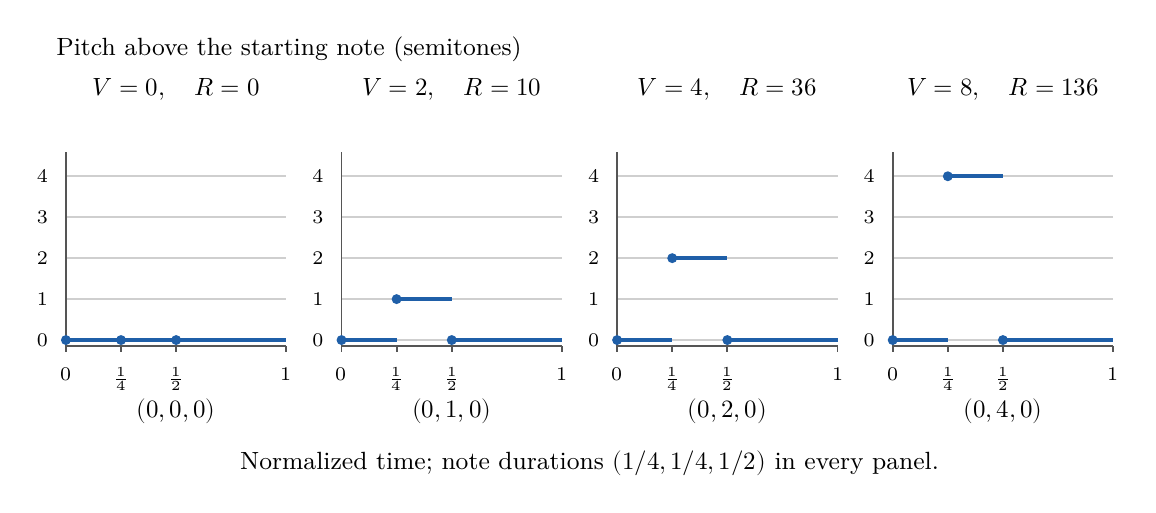
\begin{tikzpicture}[font=\small,line width=.65pt,x=1cm,y=.52cm]
\foreach \xshift/\apex/\travel/\rank in {0/0/0/0,3.5/1/2/10,7/2/4/36,10.5/4/8/136} {
 \begin{scope}[xshift=\xshift cm]
  \node[anchor=south] at (1.4,5.6) {$V=\travel,\quad R=\rank$};
  \foreach \h in {0,1,2,3,4} {
   \draw[frameline!28] (0,\h)--(2.8,\h);
   \node[anchor=east,font=\scriptsize] at (-.1,\h) {\h};
  }
  \draw[frameline] (0,-.15)--(0,4.6);
  \draw[frameline] (0,-.15)--(2.8,-.15);
  \foreach \t/\lab in {0/0,.7/{\frac14},1.4/{\frac12},2.8/1} {
   \draw[frameline] (\t,-.15)--(\t,-.28);
   \node[anchor=north,font=\scriptsize] at (\t,-.42) {$\lab$};
  }
  \draw[elemA,line width=1.6pt] (0,0)--(.7,0);
  \draw[elemA,line width=1.6pt] (.7,\apex)--(1.4,\apex);
  \draw[elemA,line width=1.6pt] (1.4,0)--(2.8,0);
  \foreach \xx/\yy in {0/0,.7/\apex,1.4/0}
   \fill[elemA] (\xx,\yy) circle (1.8pt);
  \node at (1.4,-1.75) {$(0,\apex,0)$};
 \end{scope}
}
\node[anchor=west] at (-.25,7.1) {Pitch above the starting note (semitones)};
\node at (6.65,-3) {Normalized time; note durations $(1/4,1/4,1/2)$ in every panel.};
\end{tikzpicture}
\end{document}
